Najpoznatiji vjerojatnosni grafički modeli korišteni za probleme strukturnog
predviđanja su skriveni Markovljevi modeli \engl{hidden Markov models},
Markovljev model maksimalne entropije \engl{maximum entropy Markov model} i
uvjetna slučajna polja \engl{conditional random fields}. Svaki ima svojih
prednosti. Učenje skrivenog Markovljevog modela moguće je izvesti jako brzo ako
imamo pristup velikoj količini podataka. Prijelazne vjerojatnosti $p(x_i | y_i)$
i $p(y_i | y_{i-1})$ moguće je naučiti vrlo brzo samo brojajući supojavljivanja.
Kod uvjetnih slučajnih polja lakše je opisati ulaz značajkama što omogućava
bolju generalizaciju iz manje količine podataka, ali proces učenja je
dugotrajniji. Markovljev model maksimalne entropije je po učinkovitosti između
dva modela, omogućava brzo učenje i dobru generalizaciju, ali je primijećeno da
način učenja dovodi do problema pristranosti oznakama \engl{label bias}
\citep{lafferty2001conditional}, a problem je detaljnije obrađen u potpoglavlju
\ref{ch:labelbias}.

\begin{figure}[H]
\tikzstyle{lightedge}=[<-,dotted]
\tikzstyle{mainstate}=[state,thick]
\tikzstyle{mainedge}=[<-,thick]
\tikzstyle{undirect}=[shape=rectangle,draw=black,fill=black]

\begin{subfigure}[b]{1\textwidth}
\begin{center}
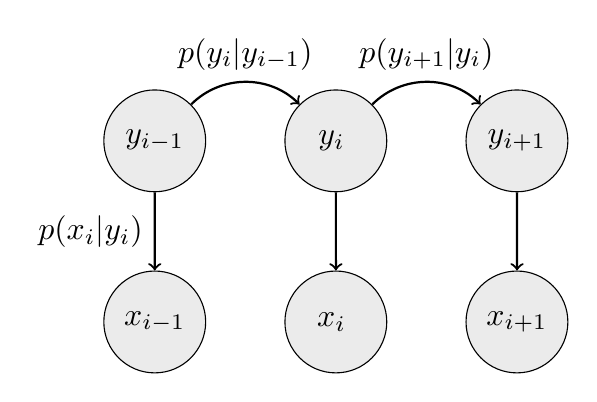
\begin{tikzpicture}[scale=1.15, every node/.style={transform shape}]
\tikzstyle{state}=[shape=circle,draw=black,fill=black!8,minimum size=32pt]
\tikzstyle{observation}=[shape=circle,draw=black,fill=black!8,minimum size=32pt]
% states
\node[state] (s1) at (0,2) {$y_{i-1}$};
\node[state] (s2) at (2,2) {$y_{i\,\,}$}
    edge [mainedge,bend right=45] node[auto,swap] {$p(y_{i}|y_{i-1})$} (s1);
\node[state] (s3) at (4,2) {$y_{i+1}$}
    edge [mainedge,bend right=45] node[auto,swap] {$p(y_{i+1}|y_{i})$} (s2);
% observations
\node[observation] (x1) at (0,0) {$x_{i-1}$}
    edge [mainedge] node[left] {$p(x_{i}|y_{i})$} (s1);
\node[observation] (x2) at (2,0) {$x_{i\,\,}$}
    edge [mainedge] (s2);
\node[observation] (x3) at (4,0) {$x_{i+1}$}
    edge [mainedge] (s3);
\end{tikzpicture}
\caption{Skriveni Markovljev model}
\label{modeli1:hmm}
\end{center}
\end{subfigure}

\begin{subfigure}[b]{0.5\textwidth}
\begin{center}
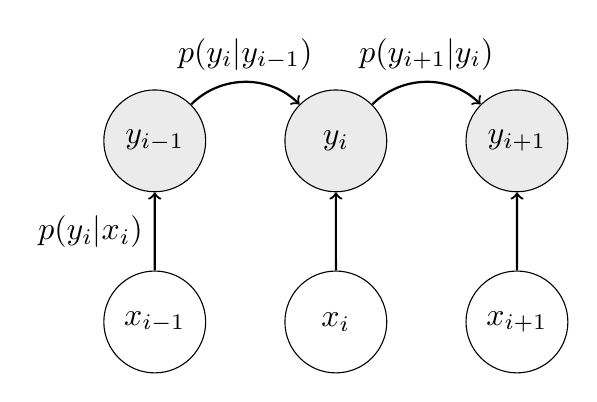
\begin{tikzpicture}[scale=1.15, every node/.style={transform shape}]
\tikzstyle{state}=[shape=circle,draw=black,fill=black!8,minimum size=32pt]
\tikzstyle{observation}=[shape=circle,draw=black,fill=white!20,minimum size=32pt]
% states
\node[state] (s1) at (0,2) {$y_{i-1}$};
\node[state] (s2) at (2,2) {$y_{i}$}
    edge [mainedge,bend right=45] node[auto,swap] {$p(y_{i}|y_{i-1})$} (s1);
\node[state] (s3) at (4,2) {$y_{i+1}$}
    edge [mainedge,bend right=45] node[auto,swap] {$p(y_{i+1}|y_{i})$} (s2);
% observations
\node[observation] (x1) at (0,0) {$x_{i-1}$}
    edge [->,thick] node[left] {$p(y_{i}|x_{i})$} (s1);
\node[observation] (x2) at (2,0) {$x_{i}$}
    edge [->,thick] (s2);
\node[observation] (x3) at (4,0) {$x_{i+1}$}
    edge [->,thick] (s3);
\end{tikzpicture}
\caption{Markovljev model maksimalne entropije}
\end{center}
\end{subfigure}
\begin{subfigure}[b]{0.5\textwidth}
\begin{center}
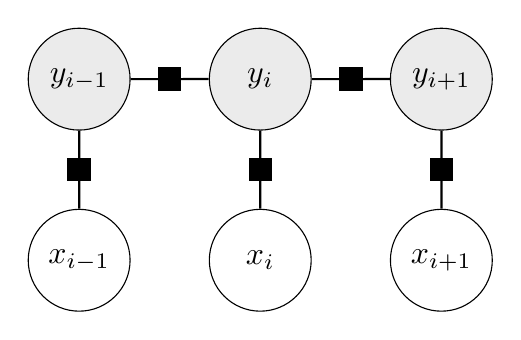
\begin{tikzpicture}[scale=1.15, every node/.style={transform shape}]
\tikzstyle{state}=[shape=circle,draw=black,fill=black!8,minimum size=32pt]
\tikzstyle{observation}=[shape=circle,draw=black,fill=white!20,minimum size=32pt]
% states
\node[state] (s1) at (0,2) {$y_{i-1}$};
\node[state] (s2) at (2,2) {$y_{i}$}
    edge [thick] node[undirect] {} (s1);
\node[state] (s3) at (4,2) {$y_{i+1}$}
    edge [thick] node[undirect] {} (s2);
% observations
\node[observation] (x1) at (0,0) {$x_{i-1}$}
    edge [thick] node[undirect] {} (s1);
\node[observation] (x2) at (2,0) {$x_{i}$}
    edge [thick] node[undirect] {} (s2);
\node[observation] (x3) at (4,0) {$x_{i+1}$}
    edge [thick] node[undirect] {} (s3);
\end{tikzpicture}
\caption{Uvjetna slučajna polja}
\end{center}
\end{subfigure}
\caption{Prikaz predložaka grafičkih modela.}
\label{fig:grafickimodeli}
\end{figure}


\subsection{Skriveni Markovljev model}

Koristi se najčešće kod problema gdje prijelazne vjerojatnosti modeliraju niz --
kao što je prikazano na slici \ref{fig:grafickimodeli}. To čini model prikladnim
za problem označavanja vrste riječi \citep{halacsy2007hunpos} i prepoznavanja
imenovanih entiteta \citep{zhou2002named}. Kako u većini slučajeva nemamo
dovoljno podataka i želimo dodati neke vanjske informacije poput toga da se
imenovani entitet koji nije bio u skupu za učenje pojavljuje u nekom rječniku
kojeg imamo ili da riječi s određenim prefiksom su češće imenice nego glagoli
onda se algoritam učenja brojanja supojavljivanja zamijenjuje Baum-Welch
algoritmom koji ima složenost $O(T M ^ k)$ -- gdje je $T$ duljina niza, $M$ broj
oznaka koje možemo predvidjeti za svaki niz i $k+1$ broj prijašnjih odluka
kojima uvjetujemo trenutnu, ali pokazalo se da algoritam jako teško dolazi do
dobrog lokalnog optimuma te se za prethodno navedene probleme ipak koriste drugi
modeli \citep{johnson2007doesn}.

\subsection{Markovljev model maksimalne entropije}

Markovljev model maksimalne entropije \engl{maximum entropy Markov model}
izravno su primijenili \citet*{mccallum2000maximum} koristeći modele maksimalne
entropije (logističke regresije) na probleme označavanja nizova. Model je vrlo
sličan skrivenom Markovljevom modelu \engl{hidden Markov model}, ali je
fleksibilniji jer omogućava veću slobodu u odabiru značajki opaženih varijabli.
Modelira se uvjetna vjerojatnost $i$-te oznake izlaza $y_i$ za dane $x$ i
prijašnje oznake $y_{i-1}$ prikazana u jednadžbi \ref{eq:maxent1}.

\begin{equation}\label{eq:maxent1}
\begin{aligned}
  p(y_i | x, y_{i-1}; \mathbf{w}) = \frac{1}{Z(x, y_{i-1}; \mathbf{w})} \exp \big[ \mathbf{w}^\top \phi(x, y_i, y_{i-1})\big] \\
  Z(x, y_{i-1}; \mathbf{w}) = \sum_{y' \in \mathcal{Y}} \exp \big[ \mathbf{w}^\top \phi(x, y', y_{i-1})\big]
\end{aligned}
\end{equation}

Model se uči koristeći prave izlazne nizove kao skup podataka za učenje i
koriste se pravi $y_{i-1}$ za generiranje primjera za učenje. Navedeni postupak
proizvede primjere za učenje višerazredne klasifikacije čiji je broj jednak
broju svih pojavljivanja u cijelom skupu za učenje. Taj generirani skup koristi
se za učenje vektora $\mathbf{w}$ postupkom koji je identičan učenju modela
maksimalne entropije -- za učenje se može koristiti neka varijanta gradijentnog
spusta.

Kod zaključivanja koristi se algoritam Viterbi za rješavanje $\argmax$ problema
(\ref{argmaxproblem}). Zbog ove kombinacije algoritama učenja i zaključivanja
dolazi do problema pristranosti oznakama (potpoglavlje \ref{ch:labelbias}).

\cite{cohen05ijcai} pokušali su smanjiti utjecaj pristranosti oznakama i
učinkovtost je usporediva s uvjetnim slučajnim poljima, ali sve prednosti vezane
uz učinkovitost učenja iščezavaju.


\subsection{Uvjetna slučajna polja}

\citet*{lafferty2001conditional} uvode uvjetna slučajna polja kao rješenje
problema pristranosti oznakama i eksperimentalno potvrđuju njegovo nepostojanje.
Problem je poznat i ranije kod primjene neuronskih Markovljevih modela na slične
probleme \citep{leon1991approche}. Uvjetna slučajna polja nemaju određenu
funkciju gubitka nego koriste log-gubitak kao aproksimaciju Hammingovog gubitka
preko cijelog strukturiranog izlaza. Zbog toga ih je moguće primijeniti samo na
probleme čija se funkcija gubitka može dekomponirati po elementima. Modelira se
uvjetna vjerojatnost prikazana u jednadžbi \ref{eq:crf}.

\begin{equation}\label{eq:crf}
\begin{aligned}
  p(y | x; \mathbf{w}) = \frac{1}{Z(x; \mathbf{w})} \exp \big[ \mathbf{w}^\top \phi(x, y)\big] \\
  Z(x; \mathbf{w}) = \sum_{y' \in \mathcal{Y}} \exp \big[ \mathbf{w}^\top \phi(x, y')\big]
\end{aligned}
\end{equation}

$Z(x; \mathbf{w})$ particijska je funkcija i sumira sve izlaze za koje model
daje kriva predviđanja. Ako se koristi iterativni algoritam učenja to znači da
za pravilnu procjenu parametara trebat ćemo računati ovu sumu svaki put prije
korigiranja težinskog vektora $\mathbf{w}$. Ta suma je u generalnom slučaju
prevelika za računati, ali ako se pretpostavi struktura linearnog lanca onda ju
je moguće izračunati koristeći dinamičko programiranje i svaka prilagodba na
novi problem koji je predstavljen netrivijalnim linearnim lancem zahtjeva novu
implementaciju algoritama \citep{lafferty2001conditional, sha2003shallow}.

Algoritam za računanje sume $Z(x; \mathbf{w})$ ima složenost $O(T M ^ k)$ i
gotovo je identičan algoritmu \textit{forward-backward}
\citep{baum1966statistical}.

Kao što je slučaj kod modela maksimalne entropije težine $\mathbf{w}$ moguće je
regularizirati i koristi se log-posteriorna distribucija preko težina opisana u
jednadžbi \ref{eq:crflog}.

\begin{equation}\label{eq:crflog}
  \log p(\mathbf{w} | \mathcal{D}; \sigma^2) = -\frac{1}{\sigma^2} {\lVert\mathbf{w}\lVert}^2 + \sum_{(x_n, y_n) \in \mathcal{D}} \bigg[ \mathbf{w}^\top \phi(x_n, y_n) - \log Z(x_n; \mathbf{w}) \bigg]
\end{equation}

Pronalaženje optimalnog vektora težina $\mathbf{w}$ rješava se na razne načine
\citep{lafferty2001conditional, sha2003shallow, sokolovska2010efficient} i
ovisno o problemu neke je moguće ili nemoguće primijeniti, a za više detalja
čitatelj se upućuje na \citep{wallach2004conditional, sutton2006introduction}.
Zaključak je da uvjetna slučajna polja možemo primijenjivati na probleme gdje
efikasno možemo izračunati $\argmax$ (\ref{argmaxproblem}) i particijsku
funkciju $Z(x; \mathbf{w})$. Strukturirani izlaz $y \in \mathcal{Y}$ mora imati
takvu dekompoziciju da možemo log-gubitkom aproksimirati Hammingov gubitak.
Unatoč ovim problemima model je našao primjene u označavanju vrste riječi
\citep{lafferty2001conditional}, prepoznavanju imenovanih entiteta
\citep{mccallum2003early, settles2004biomedical}, sažimanju dokumenata
\engl{document summarization} \citep{shen2007document}, sentiment analizi
\citep{mcdonald2007structured} itd. U svakom slučaju $\mathcal{Y}$ se
dekomponirao na niz odluka i algoritmi su se morali prilagoditi za pravilno
zaključivanje ili se odbacivanjem točnog zaključivanja koristilo aproksimativno.
